\begingroup
\setlength{\abovedisplayskip}{6pt}
\setlength{\belowdisplayskip}{6pt}
\setlength{\abovedisplayshortskip}{4pt}
\setlength{\belowdisplayshortskip}{4pt}
\setlength{\intextsep}{6pt}

\textbf{B.7.1. Input data.} I model the cantilever by its equivalent tip stiffness and use the attached motor mass as the lumped vibrating mass. I omit beam mass because neither beam density nor beam mass is supplied. Since $h$ is the bending depth for vertical bending, the second moment of area is $I=bh^3/12$.

{ % do not increment counter
\begin{center}\small\begin{tabular}{@{}lrl@{}}
\toprule\noalign{}
Quantity & Value & Unit \\
\midrule\noalign{}
$L$ & 0.568 & m \\
$E$ & 200 & GPa \\
$h$ & 3.00 & mm \\
$b$ & 37.0 & mm \\
$m$ & 0.520 & kg \\
$\zeta$ & 0.140 & 1 \\
$\hat F$ & 12.0 & mN \\
$N_0$ & 1500 & rpm \\
$N_{\mathrm{osc}}$ & 10 & oscillations \\
$N_f$ & 5000 & points \\
\bottomrule\end{tabular}\end{center}
}

\textbf{B.7.2. Beam and damping parameters.}

\textbf{(a) Section and beam stiffness.} Because the beam bends about the weak axis, the rectangular-section second moment of area is

\[
I=\frac{bh^3}{12}
 =\frac{(0.037)(0.003)^3}{12}
 =8.325\times10^{-11}\ \mathrm{m^4}
 =83.25\ \mathrm{mm^4}.
\]

The tip stiffness of a fixed-free beam is $k=3EI/L^3$. Therefore,

\[
EI=(200\times10^9)(8.325\times10^{-11})
 =16.65\ \mathrm{N\,m^2},
\qquad
k=\frac{3(16.65)}{(0.568)^3}
 =272.58\ \mathrm{N/m}.
\]

\[
\boxed{
\begin{aligned}
I&=8.325\times10^{-11}\ \mathrm{m^4},&
EI&=16.65\ \mathrm{N\,m^2},&
k&=272.58\ \mathrm{N/m}
\end{aligned}}
\qquad\text{(B.7.2.a)}
\]

\textbf{(b) Natural frequency and damping.} The natural frequency follows from the lumped mass and beam stiffness.

\[
\omega_n=\sqrt{\frac{k}{m}}
 =\sqrt{\frac{272.58}{0.520}}
 =22.895\ \mathrm{rad/s},
\qquad
f_n=\frac{\omega_n}{2\pi}=3.6439\ \mathrm{Hz}.
\]

Critical damping is $c_{\mathrm{cr}}=2m\omega_n$. Since the damping ratio is $\zeta=c/c_{\mathrm{cr}}$, the physical damping coefficient is

\[
c_{\mathrm{cr}}=2(0.520)(22.895)=23.811\ \mathrm{N\,s/m},
\qquad
c=\zeta c_{\mathrm{cr}}=(0.140)(23.811)=3.3335\ \mathrm{N\,s/m}.
\]

\[
\boxed{
\begin{aligned}
\omega_n&=22.895\ \mathrm{rad/s},&
f_n&=3.6439\ \mathrm{Hz},\\
c_{\mathrm{cr}}&=23.811\ \mathrm{N\,s/m},&
c&=3.3335\ \mathrm{N\,s/m}
\end{aligned}}
\qquad\text{(B.7.2.b)}
\]

\textbf{(c) Quasi-static deflection.} Because quasi-static loading makes the excitation frequency negligible, $\omega\to0$ while $\omega_n$ remains fixed. The force-normalized frequency response then approaches one, so

\[
u_{\mathrm{qst}}=\frac{\hat F}{k}
 =\frac{0.012}{272.58}
 =4.4024\times10^{-5}\ \mathrm{m}.
\]

\[
\boxed{u_{\mathrm{qst}}=44.024\ \mu\mathrm{m}}
\qquad\text{(B.7.2.c)}
\]

\textbf{B.7.3. Resonance quantities.}

\textbf{(a) True resonance and damped frequency.} Since $\zeta<1/\sqrt{2}$, the magnification has a nonzero maximum. Differentiating the magnification with respect to the frequency ratio gives

\[
\omega_r=\omega_n\sqrt{1-2\zeta^2}
 =22.442\ \mathrm{rad/s}.
\]

The damped natural frequency comes from the complementary solution.

\[
\omega_d=\omega_n\sqrt{1-\zeta^2}
 =22.670\ \mathrm{rad/s}.
\]

\[
\boxed{\omega_r=22.442\ \mathrm{rad/s},
\qquad
\omega_d=22.670\ \mathrm{rad/s}}
\qquad\text{(B.7.3.a)}
\]

\textbf{(b) Peak magnification.} Substituting $\omega_r$ into the magnification expression gives

\[
M_r=\frac{1}{2\zeta\sqrt{1-\zeta^2}}
 =\frac{1}{2(0.140)\sqrt{1-(0.140)^2}}
 =3.60695.
\]

\[
\boxed{M_r=3.60695}
\qquad\text{(B.7.3.b)}
\]

\textbf{(c) Magnification at phase resonance.} Phase resonance occurs when the real part of the FRF denominator is zero, which gives $\omega=\omega_n$. Thus,

\[
M_{90}=\frac{1}{2\zeta}
 =\frac{1}{2(0.140)}
 =3.57143.
\]

\[
\boxed{M_{90}=3.57143}
\qquad\text{(B.7.3.c)}
\]

\textbf{(d) Physical response at phase resonance.} At $\omega=\omega_n$, the normalized FRF is

\[
\operatorname{FRF}(\omega_n)
 =\frac{1}{2i\zeta}
 =-\frac{i}{2\zeta}.
\]

Multiplying by the quasi-static displacement gives

\[
\hat u_{90}
 =u_{\mathrm{qst}}\operatorname{FRF}(\omega_n)
 =-i\frac{u_{\mathrm{qst}}}{2\zeta}
 =-i\,157.229\ \mu\mathrm{m}.
\]

Therefore,

\[
\boxed{\hat u_{90}=-i\,157.229\ \mu\mathrm{m},
\qquad
\lvert\hat u_{90}\rvert=157.229\ \mu\mathrm{m}}
\qquad\text{(B.7.3.d)}
\]

\textbf{(e) Frequency and RPM conversions.} Since $f=\omega/(2\pi)$, division by $2\pi$ converts each angular frequency to hertz. Multiplication by $60$ then converts hertz to revolutions per minute.

\[
\begin{aligned}
f_r&=\frac{\omega_r}{2\pi}=3.57174\ \mathrm{Hz},
&N_r&=60f_r=214.305\ \mathrm{rpm},\\
f_n&=\frac{\omega_n}{2\pi}=3.64388\ \mathrm{Hz},
&N_{90}&=60f_n=218.633\ \mathrm{rpm}.
\end{aligned}
\]

\[
\boxed{
\begin{aligned}
f_r&=3.57174\ \mathrm{Hz},&N_r&=214.305\ \mathrm{rpm},\\
f_n&=3.64388\ \mathrm{Hz},&N_{90}&=218.633\ \mathrm{rpm}
\end{aligned}}
\qquad\text{(B.7.3.e)}
\]

\textbf{B.7.4. Time response at phase resonance.}

\textbf{(a) Excitation frequency.} Phase resonance uses $\omega=\omega_n$, so

\[
\boxed{\omega=22.895\ \mathrm{rad/s},
\qquad
f=\frac{\omega}{2\pi}=3.64388\ \mathrm{Hz}}
\qquad\text{(B.7.4.a)}
\]

\textbf{(b) Period.} The period of the phase-resonant oscillation is

\[
\tau=\frac{2\pi}{\omega}
 =\frac{2\pi}{22.895}
 =0.274433\ \mathrm{s}.
\]

\[
\boxed{\tau=0.274433\ \mathrm{s},
\qquad
N_{\mathrm{osc}}\tau=2.74433\ \mathrm{s}}
\qquad\text{(B.7.4.b)}
\]

\textbf{(c) Real displacement.} The physical force is taken as $F(t)=\hat F\cos(\omega_nt)$. Since $\hat u_{90}=-iU$, where

\[
U=\frac{u_{\mathrm{qst}}}{2\zeta}=157.229\ \mu\mathrm{m},
\]

the real part of the complex steady-state response is

\[
u_{\mathrm{ss}}(t)
 =\operatorname{Re}\{\hat u_{90}e^{i\omega_nt}\}
 =U\sin(\omega_nt).
\]

The assignment specifies the number of cycles but not initial conditions for this plot, so the steady-state response is the direct result. For comparison, the figure also shows the response when the force is switched on at $t=0$ and the mass starts from rest. Applying $u(0)=0$ and $\dot u(0)=0$ to the complete response gives

\[
u_{\mathrm{rest}}(t)
 =U\sin(\omega_nt)
 -\frac{U\omega_n}{\omega_d}
 e^{-\zeta\omega_nt}\sin(\omega_dt).
\]

\begin{figure}[H]
\centering
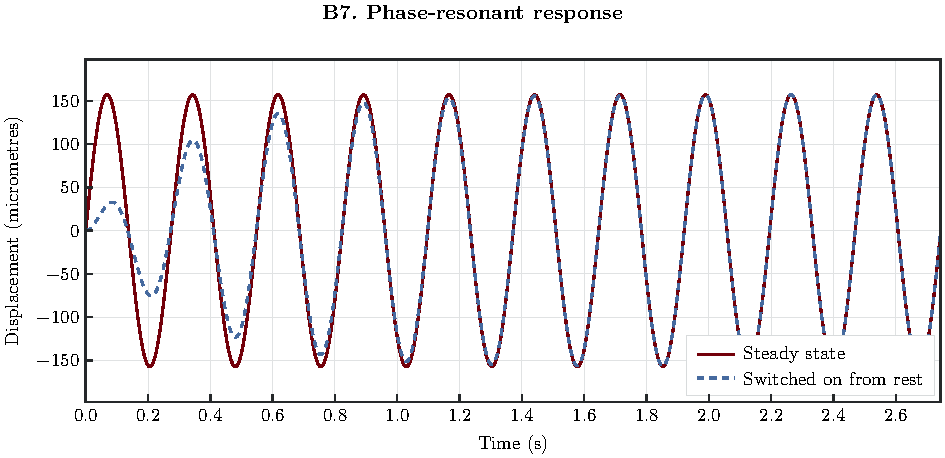
\includegraphics[width=0.95\linewidth,height=0.30\textheight,keepaspectratio,alt={B.7.4.c. Phase-resonant steady-state displacement and separately identified switched-on-from-rest response.}]{figures/generated/solutions/B7_time.pdf}
\caption{B.7.4.c. Phase-resonant real displacement over $N_{\mathrm{osc}}=10$ cycles. The dashed blue curve includes the transient required when the force is switched on from rest.}
\end{figure}

\textbf{B.7.5. Graduate work.}

\textbf{(a) Operational frequency and FRF sweep.} The operating speed is $N_0=1500\ \mathrm{rpm}$, so

\[
f_0=\frac{N_0}{60}=25.0\ \mathrm{Hz},
\qquad
\omega_0=2\pi f_0=157.080\ \mathrm{rad/s}.
\]

For the sweep, define $p=\omega/\omega_n=2\pi f/\omega_n$. The magnitude and phase are

\[
M(f)=\frac{1}{\sqrt{(1-p^2)^2+(2\zeta p)^2}},
\qquad
\phi(f)=-\operatorname{atan2}(2\zeta p,1-p^2).
\]

Using $N_f=5000$ uniformly spaced frequencies from $f=0$ to $f=f_0$ gives the magnitude and phase shown below.

\begin{figure}[H]
\centering
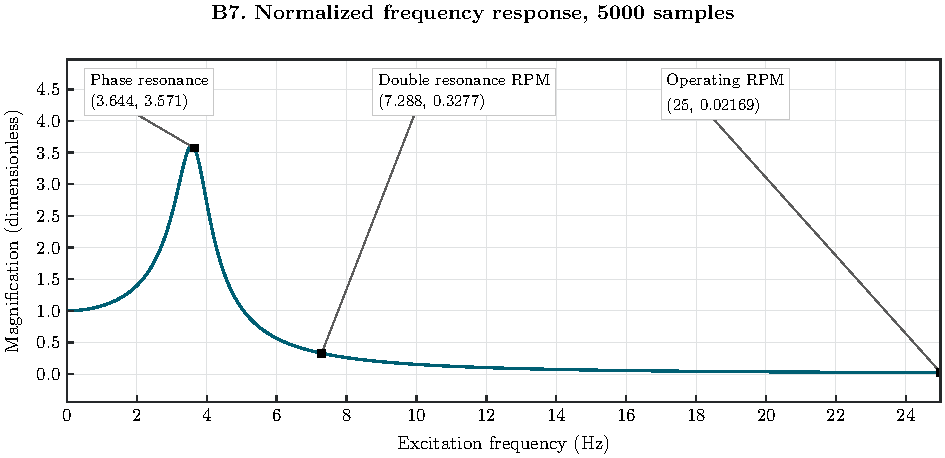
\includegraphics[width=0.95\linewidth,height=0.30\textheight,keepaspectratio,alt={B.7.5.a. Dimensionless FRF magnitude from quasi-static excitation to the operational frequency.}]{figures/generated/solutions/B7_magnitude.pdf}
\caption{B.7.5.a. Dimensionless FRF magnitude from $0$ to $f_0=25.0\ \mathrm{Hz}$.}
\end{figure}

\begin{figure}[H]
\centering
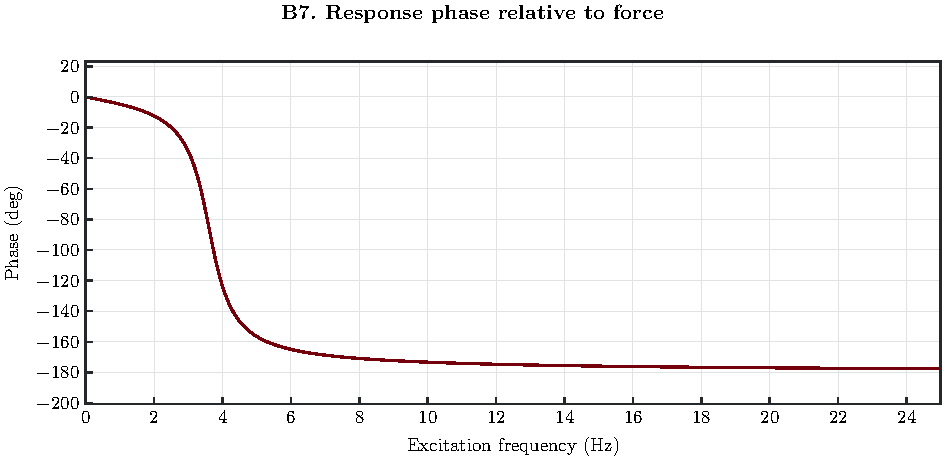
\includegraphics[width=0.95\linewidth,height=0.30\textheight,keepaspectratio,alt={B.7.5.a. FRF phase from quasi-static excitation to the operational frequency.}]{figures/generated/solutions/B7_phase.pdf}
\caption{B.7.5.a. FRF phase from $0$ to $f_0=25.0\ \mathrm{Hz}$.}
\end{figure}

\textbf{(b) Requested FRF values.} The phase-resonance speed is $N_{90}=218.633\ \mathrm{rpm}$. Doubling that speed doubles the excitation frequency, so the second requested point is $2N_{90}=437.265\ \mathrm{rpm}$ and $f=2f_n=7.28775\ \mathrm{Hz}$.

\begin{center}\small
\begin{tabular}{@{}lrrr@{}}
\toprule\noalign{}
Operating point & $f$ (Hz) & $N$ (rpm) & $\lvert\mathrm{FRF}\rvert$ \\
\midrule\noalign{}
Phase resonance & 3.64388 & 218.633 & 3.57143 \\
Double phase-resonance speed & 7.28775 & 437.265 & 0.32767 \\
Operational speed & 25.0000 & 1500.000 & 0.02169 \\
\bottomrule
\end{tabular}
\end{center}

\textbf{(c) Operational vibration magnitude.} At $f_0=25.0\ \mathrm{Hz}$, the frequency ratio is $p_0=\omega_0/\omega_n=6.86082$. Therefore,

\[
\lvert\hat u_0\rvert
 =u_{\mathrm{qst}}M(f_0)
 =(44.024\ \mu\mathrm{m})(0.0216868)
 =0.954744\ \mu\mathrm{m}.
\]

\[
\boxed{\lvert\hat u_0\rvert=0.954744\ \mu\mathrm{m}}
\qquad\text{(B.7.5.c)}
\]

\textbf{(d) Run-up interpretation.} When the motor starts, the displacement contains a transient because the mass begins away from the eventual forced steady state. As the motor accelerates, the excitation frequency passes through true resonance near $N_r=214.305\ \mathrm{rpm}$, where the steady-state magnification is largest. Phase resonance occurs slightly later at $N_{90}=218.633\ \mathrm{rpm}$, so the two speeds are close but not identical.

After the motor passes this region, the FRF magnitude decreases and the displacement becomes small at the operational speed. Under the supplied constant force amplitude, the predicted steady-state magnitude decreases from about $157\ \mu\mathrm{m}$ near phase resonance to $0.955\ \mu\mathrm{m}$ at $1500\ \mathrm{rpm}$. The actual maximum during acceleration also depends on how quickly the motor crosses resonance. A rotating imbalance normally produces a force that varies with speed squared, so the fixed-$\hat F$ sweep describes the structural FRF and does not by itself predict the complete transient run-up.

\clearpage
\matlabcaption{Time response and FRF plots for B.7.}

\lstinputlisting[style=hwmatlab]{matlab/B7.m}

\endgroup
